% Procedure is the first result subsection; this figure alone spans both columns.
\WIPsubsection{Annotated Procedure}
The main comparison included seven annotated procedures. \Cref{fig:procedure} shows dissection, repair phases, stitches, and elapsed time for each recording. Median procedure duration was 115.91 minutes with 3 mm instruments and 75.46 minutes with 8 mm instruments (\cref{tab:sutures}). Procedure duration ended at the final suture-cutting event.

\begin{figure*}[t]
\centering
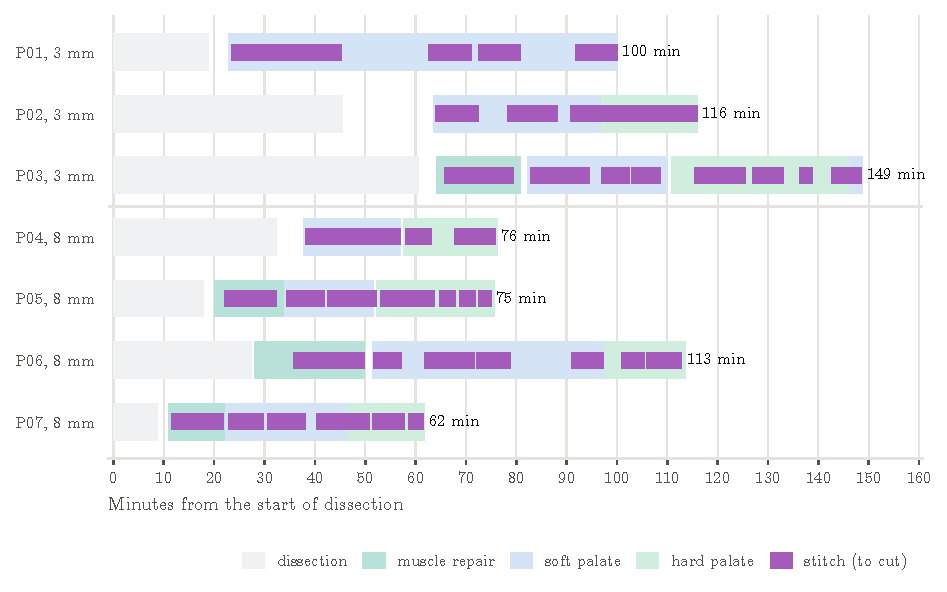
\includegraphics[width=\textwidth]{figures/results/procedure.pdf}
\caption{Procedure timelines aligned at dissection onset. Shading indicates operative phases; purple bars show sutures through cutting. Right-hand values give duration in minutes, including pauses.}
\label{fig:procedure}
\end{figure*}
